% 4 Gjennomførbarhetsanalyse
\section{Gjennomførbarhetsanalyse}

% 4.1 Tilgjengelige ressurser
\subsection{Tilgjengelige ressurser}

\subsubsection{Utstyr}
Alle gruppemedlemmer har en egen PC som kjører Windows, Linux eller macOS. Det kreves ingen spesielt utstyr for gjennomføring av prosjektet. 

\subsubsection{Kunnskaper}
For å kunne effektivt planlegge og gjennomføre prosjektarbeid er det ønskelig at studenten har: 

\begin{itemize}
    \item generelle programmeringskunnskaper 
    \item kjennskap til objektorientert programmeringsspråk, som Java eller Kotlin
    \item kjennskap til systemutvikling
    \item kjennskap til utvikling av tjenester etter REST prinsippet
    \item kjennskap til kvalitetssikring av programkode ved hjelp av enhetstester
    \item kjennskap til bruk av agile utviklingsmetodikker
    \item kjennskap til bruk av Jira Software
    \item kjennskap til bruk av Git og GitHub
\end{itemize} 

\subsubsection{Litteratur}
Det er planlagt å bruke ulike informasjonskilder slik som bøker, Internett kilder, interne dokumenter og rapporter osv. For å kunne finne inspirasjon eller mer elegante løsninger kan det være aktuelt å bruke YouTube, Stackoverflow og informasjon fra forskjellige kurser / plattformer.

% 4.2 Risikoanalyse
\newpage
\subsection{Risikoanalyse}

\subsubsection{Bakgrunn for risikoanalyse}

I starten av hvert prosjekt er det viktig å vurdere mulig risiko som kan oppstå underveis. Godt utført risikoanalyse gir prosjektgruppe en bedre oversikt over problemer, som kan oppstå under prosjektgjennomføringen. Dette gir mulighet til å iverksette risikoreduserende tiltak i tide og minimere risiko for å ikke fullføre prosjektet \cite{4-forelesning-risikonalyse}.

Det ble laget en risiko tabell som viser en oversikt over mulige uønskede hendelser. Sannsynlighet og konsekvens vurderes for hver enkelt hendelse. Ved hjelp av en enkel formel beregnes det grad av risiko for gjennomføring av prosjektet. Ut fra resultater kan man vurdere behov for iverksetting av risikoreduserende tiltak \cite{4-forelesning-risikonalyse}.    

\subsubsection*{Begreper}

Uønsket hendelse er en hendelse som kan føre til tap av verdier \cite{4-norsk-standard}.\\  
Risiko er en kombinasjon av sannsynlighet og konsekvens for en uønsket hendelse \cite{4-norsk-standard}.\\
Sannsynlighet viser i hvilken grad er det trolig at en bestemt hendelse vil inntreffe \cite{4-norsk-standard}.\\  
Konsekvens viser mulig følge av en bestemt hendelse \cite{4-norsk-standard}.
 
\begin{table}[H]
\centering
\begin{tabular}{|c|c|} 
\hline
Sannsynlighet & Beskrivelse\\
\hline\hline
1 & veldig lite sannsynlig\\
\hline
2 & mindre sannsynlig\\
\hline
3 & sannsynlig\\
\hline
4 & meget sannsynlig\\
\hline
5 & svært sannsynlig\\
\hline
\end{tabular}
\caption{Grad av sannsynlighet \cite{4-forelesning-risikonalyse}}
\label{table1}
\end{table}

\begin{table}[H]
\centering
\begin{tabular}{|c|c|} 
\hline
Konsekvens & Beskrivelse\\
\hline\hline
1 & ikke farlig\\
\hline
2 & farlig\\
\hline
3 & kritisk\\
\hline
4 & meget kritisk\\
\hline
5 & katastrofalt\\
\hline
\end{tabular}
\caption{Grad av konsekvens \cite{4-forelesning-risikonalyse}}
\label{table2}
\end{table} 

\subsubsection*{Beregning av risikonivå}

Risiko(h) = Sannsynlighet(h) * Konsekvens(h),\\ hvor h - hendelse \cite{4-forelesning-risikonalyse}  

%TABLE - PART - ONE
\begin{landscape}
\subsubsection{Risikoanalyse}
\begin{table}[H]
\begin{tabular}{|c|p{4cm}|c|c|c|c|p{4cm}|p{4cm}|}    
\hline
Nr. & Beskrivelse av hendelsen & Påvirker & Sannsynlighet & Konsekvens & Risikonivå & Forebyggende tiltak & Korrigerende tiltak  \\
\hline\hline
1 & Prosjektet ble ikke startet innen den gitte tidsrammen & Prosjekt & 2 & 2 & 4 & Oppstart møte. Velge kommunikasjons verktøy. Etablere arbeidsplan og rutiner. & Ved behov sette litt ekstra tid for å starte å jobbe med prosjektet i tide. \\
\hline
2 & Prosjektet ble ikke fullført innen den gitte tidsrammen & Prosjekt & 3 & 4 & 12 & Aktivt bruk av smidige utviklingsmetoder i løpet av hele prosjektperioden. Ha kontroll over utførelsen av ulike aktiviteter. God kommunikasjon mellom gruppemedlemmer og veiledere.  & Ta kontakt med oppdragsgiver og veiledere for å justere arbeidsplan. Diskutere mulighet for gjennomføring av manglende aktiviteter i et annet prosjekt.   \\
\hline
3 & Sykdom eller skade i en gruppe & Person / Prosjekt & 4 & 2 & 8 & Unngå alvorlig sykdom og redusere aktiviteter, som kan føre til skade. & De andre gruppemedlemmer hjelper ved behov  \\
\hline
4 & Dobbeltarbeid & Person / Prosjekt & 2 & 2 & 4 & God kommunikasjon mellom gruppemedlemmer. Utarbeide og følge arbeidsplan. Aktivt bruk av Jira Software (Scrum).    & Gjøre nødvendige justeringer i arbeidsplanen. Utføre de kritiske aktivitetene. Omprioritering av aktiviteter ved behov.  \\
\hline
\end{tabular}
\caption{Risikotabell (del 1) som viser mulige uønskede hendelser, grad av sannsynlighet, grad av konsekvens, beregnet risikonivå og mulige tiltak \cite{4-forelesning-risikonalyse}.}
\label{table}
\end{table}
\end{landscape}

%TABLE - PART - ONE
\begin{landscape}
\begin{table}[H]
\begin{tabular}{|c|p{4cm}|c|c|c|c|p{4cm}|p{4cm}|}   
\hline
Nr. & Beskrivelse av hendelsen & Påvirker & Sannsynlighet & Konsekvens & Risikonivå & Forebyggende tiltak & Korrigerende tiltak \\
\hline\hline
5 & Dårlig arbeidsmiljø i en gruppe / Konflikter & Person / Prosjekt & 1 & 4 & 4 & Fordeling av roller og ansvarsområder i en gruppe. God kommunikasjon for å forebygge mulige konfliktsituasjoner. & Ved oppstått misforståelse prøve å finne årsaken til dette. Etterpå finne en generell løsning til problemet. For eksempel, gjøre endringer i ansvarsområdet, justere arbeidsmengde osv. \\
\hline
6 & Tap av rapport, kildekode, dokumentasjon o.l. & Produkt / Prosjekt & 2 & 5 & 10 & Dokumentasjon og kildekode skal lagres både lokalt hos alle gruppemedlemmer og på de valgte sky tjenester som GitHub, Overleaf osv. & Prøve å gjenopprette tapt dokumentasjon og kildekode. Ved behov starte på nytt fra siste checkpoint. \\
\hline
7 & Ønsket funksjonalitet blir ikke implementert & Produkt / Prosjekt & 2 & 4 & 8 & Under planlegging av prosjektarbeid bør gruppe sette realistiske mål over funksjonalitet som skal bli implementert i applikasjonen. & Gjøre endringer i prosjektplanen. Prøve å finne alternative løsninger. Prioritering av oppgaver. \\
\hline
\end{tabular}
\caption{Risiko tabell (del 2) som viser mulige uønskede hendelser, grad av sannsynlighet, grad av konsekvens, beregnet risikonivå og mulige tiltak \cite{4-forelesning-risikonalyse}.}
\label{table}
\end{table}
\end{landscape}

\subsubsection{Risikomatrise}

Risiko kan fremstilles ved hjelp av en risiko matrise, der sannsynlighet er plassert langs x – aksen og konsekvens langs y – aksen.
Risiko matrise er delt inn i grønt, gul og rødt farge som representerer henholdsvis lavt, middels og høyt risikonivå for en bestemt hendelse i risiko tabellen.
Tabellen risiko akseptkriterier viser behov for igangsettelse av risikoreduserende tiltak i forhold til risikonivå.

\begin{figure}[h]
\centering
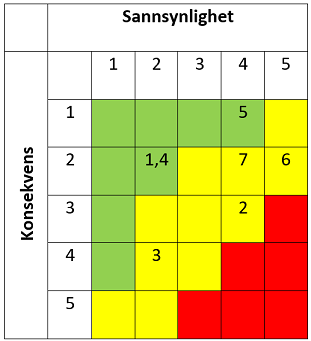
\includegraphics{images/risikomatrise2.png}
\caption{Risikomatrise}
\label{figur1}
\end{figure}
 

\begin{table}[h]
\centering
\begin{tabular}{|c|c|} 
\hline
Nivå & Tiltak\\
\hline\hline
Lavt & Aksepteres. \\
\hline
Middels & Aksepteres. Kontinuerlig utførelse av risikoreduserende tiltak.  \\
\hline
Høyt & Aksepteres ikke. Risikoreduserende tiltak skal utføres umiddelbart.\\
\hline 
\end{tabular}
\caption{Risikoakseptkriterier}
\label{table5}
\end{table} 

\
% 4.3 Drøfting og vurdering av ulike løsningsmetoder og analyse av forslag
\newpage
\subsection{Drøfting og vurdering av ulike løsningsmetoder og analyse av forslag}

\subsubsection{Programmering verktøy / Utviklingsverktøy}
Det finnes mange forskjellige programmering verktøy. Følgende er beskrivelse av teknologier som er aktuelt i vårt prosjekt.

\subsubsection*{Programmeringsspråk}

Prosjektgruppe har valgt å bruke Kotlin som programmeringsspråk. Grunnen til dette er at applikasjonen skal lages ved hjelp av Ktor rammeverket. Og det er bare Kotlin som kan bli brukt til dette formålet. Dersom prosjektgruppen velger et annet rammeverk, for eksempel Spring Boot, kan Java bli et godt alternativ.

Kotlin er et moderne programmeringsspråk. Kotlin er utviklet av JetBrains som mål å være et bedre alternativ til Java. Kotlin tilbyr en moderne syntaks, mer funksjonell paradigme i form av f.eks. funksjoner som verdier og funksjoner av høyere orden. Kotlin har null verdier som en del av type systemet, en verdi kan aldri være eksplisitt null uten håndtering. Kotlin byr på mye mer enn dette også, i sum gjør det Kotlin til et godt valg over Java \cite{4-imaginarycloud.com}.

\subsubsection*{Web Rammeverk}

Det finnes flere rammeverk som brukes til å skrive applikasjoner i Kotlin. Prosjektgruppe har bestemt seg for å utvikle applikasjonen som REST tjeneste med Ktor rammeverket av JetBrains.

Ktor er et asynkront mikro rammeverk som egner seg godt til utvikling av applikasjoner i Kotlin. Både Kotlin, Ktor og IntelliJ IDEA er produkter laget av JetBrains. Dette gir et utmerket verktøy støtte for prosjekter. Det kreves ikke så mye for å lage Ktor applikasjon, legge til ønsket funksjonalitet, endre konfigurasjon osv \cite{4-ktor.io-idea}.

Ktor er lett og fleksibelt mikro rammeverk. Ved behov kan applikasjonens funksjonalitet enkelt utvides ved hjelp av plugins \cite{4-ktor.io}.

Kotlin er det eneste programmeringsspråk som kan brukes for utvikling av applikasjoner ved hjelp av Ktor rammeverket.

Spring Boot er fortsatt ledende rammeverk for utvikling av applikasjoner i Java. Den er godt dokumentert og er mye brukt blant utviklere. Dersom prosjektgruppe hadde valgt Java som programmeringsspråk, kunne Spring Boot være et godt alternativ til Ktor.
\subsubsection*{IDE (Integrated Development Environment)}

Prosjektgruppen er godt kjent med IntelliJ IDEA siden den ble mye brukt i løpet av studiet. Samtidig skal applikasjonen utvikles i Kotlin, og oppdragsgiveren prioriterer dette utviklingsmiljø også. Derfor ble den valgt for prosjektet vårt.  

IntelliJ IDEA (Community Edition) er open source IDE, som egner seg best til utvikling av Kotlin applikasjoner. IntelliJ IDEA er utviklet og vedlikeholdt av JetBrains, har flere funksjoner og er godt egnet for rask programvareutvikling. Den har også gode muligheter for integrasjon med andre typer verktøy som Git og GitHub, Gradle og Docker Compose. Siden det er ikke en god støtte for å utvikle Kotlin prosjekter i en annen IDE, finnes det ikke et bedre alternativ til IntelliJ IDEA \cite{4-jetbrains.com}.  

\subsubsection*{Dev/deployment env}
 
Prosjektgruppe har en god erfaring med bruk av Docker og Docker Compose, og derfor ble den valgt for prosjektet vårt.

Docker er et verktøy som brukes til utvikling, testing og kjøring av applikasjoner i Docker containere. Docker image inneholder alle nødvendige biblioteker, konfigurasjons filer og avhengigheter som kreves for å kunne kjøre applikasjonen \cite{4-cloudacademy.com}.

Docker Compose er et verktøy som brukes til å konfigurere og starte flere containere samtidig \cite{4-kode24.no}.

Det er flere fordeler ved bruk av Docker i programvareutvikling. Docker kan installeres på alle moderne operative systemer, har kort oppstart tid, lav innvirkning på OS og bruker ikke så mye plass på harddisken \cite{4-docker.com}.

Docker containere er portable og derfor kan bli enkelt flyttet og distribuert mellom ulike maskiner. Dette gir et stabilt kjøre miljø for applikasjonen \cite{4-circleci.com}.

Som et alternativ kan man vurdere bruk av virtuelle maskiner. I motsetning til Docker, det er flere ulemper enn fordeler med disse. Virtuelle maskiner har større innvirkning på OS, tregere og tar mye diskplass \cite{4-docker.com}.

I motsetning til Docker containere, innkapsler virtuelle maskiner en hel maskin, som gjør deling, ombygning og distribusjon av kode utfordrende. Men virtuelle maskiner har bedre sikkerhet enn Docker containere \cite{4-circleci.com}.

I enkelte prosjekter kan det være lurt å kombinere bruk av virtuelle maskiner og Docker containere \cite{4-circleci.com}.
\subsubsection*{Relasjonsdatabase}
 
Det finnes mange forskjellige typer databaser, både NoSQL og SQL. Oppdragsgiveren prioriterer bruk av MySQL database. Derfor ble den valgt for prosjektet vårt.

\subsubsection{Prosjektstyring verktøy}

\subsubsection*{Microsoft Teams}

Alle gruppemedlemmer er godt kjent med Microsoft Teams. Derfor ble den valgt som kommunikasjons verktøy for hele prosjektperioden. Det ble etablert egen Teams gruppe. Microsoft Teams støtter organisering av møter via chat, videochat, lagring av filer og integrasjon med enkelte applikasjoner \cite{4-microsoft-teams}.

\subsubsection*{Jira Software vs Trello}

Både Jira og Trello er populære agile prosjektstyring verktøy. Begge to eies av Atlassian. Hver plattform har distinkte fordeler og ulemper og kan bli brukt i ulike tilfeller. Følgende er beskrivelse av hovedforskjeller ved disse to plattformer.

Jira er godt egnet til styring av prosjekter av type programvareutvikling. Den har flere smidige funksjoner, som kan brukes under prosjektarbeid. Blant disse er mulighet til å lage Sprints, Epics og User Stories, bruk av Markup language og labels, mulighet til å legge til filer og koble prosjektet til Git repositorier \cite{4-atlassian.com-jira}.

Jira Software støtter både Scrum og Kanban prosjekter, og er det mest populære verktøyet for Scrum Teams. Scrum Board er delt inn i tre hoveddeler: TO DO, IN PROGRESS og DONE. Denne inndelingen gir godt oversikt over prosjektets arbeidsflyt, bidrar til bedre kommunikasjon mellom gruppemedlemmer og fordeling av arbeidsoppgaver \cite{4-atlassian.com-jira}.

Trello er et enkelt verktøy som er basert på Kanban board \cite{4-trello.com}. Den kan bli brukt for å visualisere ulike arbeidsflyt, men er ikke nok til å støtte store kompliserte prosjekter av type programvareutvikling \cite{4-technologyadvice.com}.

\subsubsection*{Git og GitHub vs BitBucket}

Alle gruppemedlemmer har en god erfaring med bruk av Git og GitHub siden det ble mye brukt i løpet av studiet. Derfor ble Git valgt som versjonskontroll system og GitHub som hosting for prosjektet vårt. En av de andre alternativene til lagring av kildekode er Bitbucket.

GitHub er fortsatt den største hosting for Git repository, og betjener et stort antall programvare utviklere med åpen kildekode. GitHub egner seg godt for store prosjekter, og har mulighet til å lage både offentlige og private repositorier \cite{4-geeksforgeeks.org}.

GitHub støtter prosjekter som bruker Git versjonskontroll system, og lar utviklere å jobbe sammen om et prosjekt. Den inneholder et stort antall funksjoner som gjør prosjektarbeid enklere. For eksempel, Github støtter Markdown og kan brukes til skriving av rapporter og annen dokumentasjon. GitHub kan også integreres med Jira som er et viktig verktøy for styring av prosjektarbeid \cite{4-geeksforgeeks.org}.

Bitbucket er en annen hosting som blir mer og mer populært blant utviklere. I utgangspunktet Bitbucket er fokusert på små prosjekter og lukket kildekode. Den støtter Git og Mercurial. Bitbucket integreres godt med Jira og Trello siden begge produktene er fra Atlassian \cite{4-geeksforgeeks.org}.

\subsubsection{Utviklingsmetoder / metodikker}

Det finnes to populære agile utviklingsmetoder: Scrum og Kanban. Begge to har lignende prinsipper og brukes til styring av prosjektarbeid.

\subsubsection*{Scrum}

Scrum er en metode som egner seg godt for store utviklingsprosjekter. Den består av tre deler: roller, hendelser og artefakter. Scrum Team er relativt stor og har rollefordeling: Project Owner, Scrum Master og Developers. Hver eneste person i prosjektgruppe har sitt eget ansvarsområde. Utviklingsprosess er delt inn i korte perioder med en fast lengde, sprinter. Hver Sprint består av Sprint Planning, Sprint med Daily Scrum, Sprint Review og Sprint Retrospective. Hver del av sprinten har sitt eget mål og utførelsesteknikk. I løpet av sprinten utarbeides det såkalte artefakter: Produkt Backlog, Sprint Backlog og Product Increment \cite{4-atlassian.com-kanban-vs-scrum}. 

\subsubsection*{Kanban}

Kanban er en annen utviklingsmetode. I motsetning til Scrum, egner den seg godt for mindre prosjekter. Kanban har ingen rollefordeling. Den er ikke inndelt i sprinter, og derfor mer fleksibelt enn Scrum. Kanban brukes til å visualisere kontinuerlig arbeidsflyt \cite{4-atlassian.com-kanban-vs-scrum}.
 
\subsubsection*{Scrumban}

Prosjektgruppe har bestemt seg til å bruke det beste av begge metodene og valgt Scrumban, som er en hybrid av Scrum og Kanban. I likhet med Scrum, har Scrumban iterasjoner, der prosjektgruppe jobber med prioriterte oppgaver fra Backlog. Scrumban er mye mer fleksibelt enn Scrum, og Backloggen kan utvides med nye elementer i løpet av iterasjonen. Alle møtene er «on demand» og holdes når prosjektgruppen ser behov for det. Scrumban krever ikke så mye dokumentasjon enn Scrum, og dermed sparer tid som kan bli brukt til produktutvikling \cite{4-logrocket.com-scrumban}.

Prosjektgruppe bruker Kanban board for visualisering av arbeidsflyt og setter en grense for antall elementer som kan være i «in progress» tilstand. Dette hjelper med å finne «svakheter» i gruppens arbeid, øker effektiviteten og reduserer sjansene for å ikke fullføre planlagt arbeid \cite{4-atlassian.com-wip-limits}.

\subsubsection{Dokumentasjon}

Alt prosjektarbeid skal bli godt dokumentert. Gjennom hele prosjektperioden skal det lages forskjellige rapporter, grafer og diagrammer.

\subsubsection*{Markdown vs Microsoft Word, Endnote}

Det finnes flere måter å skrive en rapport på. Tradisjonelt ble Microsoft Word og Endnote brukt til dette formål i løpet av studiet. Prosjektgruppe har valgt å bruke Markdown til å skrive rapporter og andre dokumenter i forbindelse med gjennomføring av prosjektet. En av grunnene er at GitHub som brukes til lagring av kildekode, støtter skriving og formatering av tekst i Markdown.

Selv om bruk av Markdown kan se vanskeligere for nybegynnere, den er stort sett mye bedre enn Microsoft Word. Først gjelder det dokument deling, der flere medlemmer kan skrive rapport samtidig. Det er mulig å lage en ny .md dokument i GitHub og dele den med de andre deltakere.

Ved å kombinere vanlig tekst med Markup symboler kan man style og strukturere teksten, legge til bilder, referanser, lage lister og tabeller mm. Det kan ta litt tid til å bli kjent med disse kommandoene, men det er absolutt verdt det.
Det er også mulig å nevne en bestemt person eller en gruppe på GitHub ved å skrive @ foran navnet. Ved hjelp av Git kan man spore endringer i dokumentet eller gå til en tidligere versjon \cite{4-docs.github.com}.

Microsoft Word er mye enklere i bruk og har bedre sjekk for grammatiske og stavefeil enn Markdown, GitHub. Derfor er det gunstig å sjekke teksten i Microsoft Word før den skal overføres til GitHib. I tillegg til Microsoft Word kan man bruke Endnote for å styre referanser \cite{4-endnote.com}.  

\subsubsection*{Mermaid vs VisualParadigm}
 
Prosjektgruppe skal hovedsakelig bruke Mermaid for å lage forskjellige grafer og diagrammer. Mermaid er et JavaScript-basert verktøy, som bruker enkle kommandoer for å lage kompliserte diagrammer i Markdown og endre dem dynamisk. Ved hjelp av Mermaid kan man lage flowchart, sequence diagram, class diagram, gantt diagram, pie chart diagram, entity relationship diagram osv. Mermaid er integrert i GitHub, og det er mulig å lage grafer i GitHub’s README.md fil som kan bli aktuelt i vårt prosjekt. Det finnes også Mermaid plugins for mange andre tjenester, for eksempel Visual Studio Code og IntelliJ IDEA \cite{4-mermaid.js.org}.

VisualParadigm er en alternativ type verktøy som kan bli brukt til å lage ulike diagrammer. Ved hjelp av VisualParadigm kan man lage flowchart, UML class diagrams, use case diagrams, entity relationship diagrams, grafisk fremstilling av arbeidsflyten osv. Den inneholder en stor samling av ulike maler, som kunne bli brukt i prosjektet. Men ikke alle funksjonene er gratis, og den er heller ikke koblet til GitHub. Derfor vil bruk av Mermaid prioriteres \cite{4-visual-paradigm.com}.

\subsubsection*{Jira Software}

Styring av prosjektarbeid skal gjennomføres ved hjelp av Jira Software. Prosjektgruppe skal lage et Kanban prosjekt som bruker Roadmap og Kanban board for visualisering av arbeidsflyt. Jira Software skal også brukes til generering av diverse rapporter og diagrammer som dokumenterer prosjektarbeid \cite{4-atlassian.com-jira}.

\subsubsection*{Microsoft Excel}

Microsoft Excel skal brukes til å lage og føre projektdagbok som gir en oversikt over brukt tid for hele prosjektet og forskjellige del aktiviteter samt viser detaljert beskrivelse av utført arbeid. Excel kan også benyttes til grafisk representering av prosjektarbeid, for eksempel gantt-diagram, sektor diagram osv.
% 4.4 Valg av løsning og utviklingsmetodikk
\newpage
\subsection{Valg av løsning og utviklingsmetodikk}

\subsubsection*{Programmering}

\begin{itemize}
\item Programmeringsspråk: Kotlin
\item IDE: IntelliJ IDEA
\item Rammeverk: Ktor med Arrow
\item Docker containers / Docker Compose
\item Relasjondatabase: MySQL
\end{itemize}
I seksjon 4.3 er verktøyene og alternative verktøy beskrevet og satt opp mot hverandre. Den kvalitative årsaken til valgt teknologi er at det er den teknologien team for kvalitetsregister bruker til tjeneste per dags dato, og er dermed teknologi teamet kan overta, vedlikeholde og videreutvikle etter endt oppgave.

\subsubsection*{Prosjektstyring}

\begin{itemize}
\item Kommunikasjon verktøy: Microsoft Teams
\item Prosjektstyring verktøy: Jira Software
\item Versjonskontrollverktøy: Git og Github
\end{itemize}
Dette er vertkøy vi er komfortabel med å bruke til prosjektarbeid, og er derfor et naturlig valg til dette prosjektet. Kristian jobber med Jira i sin jobb og har erfaring med det. Teams er standard løsning for kommunikasjon levert av UiT for studenter. Git er en akseptert bransjestandard for versjonskontroll av kode.
\subsubsection*{Dokumentasjon}

\begin{itemize}
\item Rapportskriving: LaTex / Markdown
\item Grafer og diagrammer: Mermaid, Jira Software, Microsoft Excel
\end{itemize}
Latex gir stor kontroll for skriving av dokumenter, samtidig som den støtter bibtex filer som gjør at det er meget lett og holde styr på referanser, og eventuelt endre referanse stil ved ønske/behov. Det gjør det også lett å overføre referanser til eventuelt andre dokumenter. Mermaidjs tilbyr en enkel deklarativ måte å definere diagrammer på som støtter versjonskontroll via Git.
\subsubsection*{Prosjektutvikling}

\begin{itemize}
    \item Utviklingsmetode: Scrumban
\end{itemize}
Scrumban er en utviklingsmetode som kombinerer både Scrum og Kanban. Scrumban ble valgt fordi den er mer fleksibel enn Scrum, krever mindre dokumentasjon og dermed sparer tid som kan brukes til prosjektutvikling. Denne metoden bruker Kanban board til visualisering av arbeidsflyt og fordeling av arbeidsoppgaver. Den egner seg best til arbeid i mindre grupper.

 

